%% Author_tex.tex
%% V1.0
%% 2012/13/12
%% developed by Techset
%%
%% This file describes the coding for rstrans.cls

\documentclass[openacc]{rstransa}%%%%where rstrans is the template name

%%%% *** Do not adjust lengths that control margins, column widths, etc. ***

%%%%%%%%%%% Defining Enunciations  %%%%%%%%%%%
% \newtheorem{theorem}{\bf Theorem}[section]
% \newtheorem{condition}{\bf Condition}[section]
% \newtheorem{corollary}{\bf Corollary}[section]
%%%%%%%%%%%%%%%%%%%%%%%%%%%%%%%%%%%%%%%%%%%%%%%

%%%% Additional packages
% \usepackage{todonotes}
\usepackage[nopar]{kantlipsum}
\usepackage{algorithm}
\usepackage{algpseudocode}

\usepackage{pgfplots}
\DeclareUnicodeCharacter{2212}{−}
\usepgfplotslibrary{groupplots,dateplot}
\pgfplotsset{compat=newest}
\usepackage{tikz}
\usetikzlibrary{positioning, backgrounds, decorations, arrows, arrows.meta, patterns, shapes, fit}
\tikzset{>=latex}
\usepackage{forest}

\usepackage{subcaption}
\usepackage{tabularray}
\usepackage{siunitx}
\sisetup{round-mode=places,round-precision=2}

%%%% Please insert respective article type here %%%%
\titlehead{Research}

\begin{document}

%%%% Article title to be placed here
\title{Zobrist Hash-based Duplicate Detection in Symbolic Regression}
\author{Bogdan Burlacu}

%%%% Insert author address here
\address{University of Applied Sciences Upper Austria\\
Heuristic and Evolutionary Algorithms Laboratory\\
Softwarepark 11, 4232, Hagenberg, Austria}

%%%% Subject entries to be placed here %%%%
\subject{xxxxx, xxxxx, xxxx}

%%%% Keyword entries to be placed here %%%%
\keywords{xxxx, xxxx, xxxx}

%%%% Insert corresponding author and its email address}
\corres{Bogdan Burlacu\\
\email{bogdan.burlacu@fh-ooe.at}}

\def\CPP{C\raisebox{0.5ex}{\tiny\textbf{++}}}

%%%% Abstract text to be placed here %%%%%%%%%%%%
\begin{abstract}
    \kant[1-2]
    % The evolutionary search in genetic programming may visit the same points in solution space multiple times, which affects efficiency and overall odds of convergence. This work introduces a method for avoiding duplicate exploration through an efficient detection mechanism for already seen solutions, based on the concept of Zobrist hashing. This type of hashing, frequently used in abstract board games, allows the efficient construction and subsequent update of transposition tables (essentially, a cache of previously seen solutions) during the run, thus providing the ability to detect duplicates during the recombination phase of the evolutionary algorithm.
    % We prototype this idea using the open-source symbolic regression library Operon and perform empirical testing on a number of synthetic and real-world datasets. Furthermore, we investigate the ability of the Zobrist-based approach to cover an artificial set of solution points generated exhaustively by a deterministic approach. The results show that our approach provides a reliable way of avoiding the evaluation of duplicate solutions during the search, with a moderate amount of overhead.
\end{abstract}
%%%%%%%%%%%%%%%%%%%%%%%%%%%

%%%%%%%%%% Insert the texts which can accomdate on firstpage in the tag "fmtext" %%%%%

% \begin{fmtext}

% \end{fmtext}

% %%%%%%%%%%%%%%% End of first page %%%%%%%%%%%%%%%%%%%%%

\maketitle

\section{Introduction}

Symbolic Regression (SR) has been rapidly emerging as a key approach in machine learning in recent years due to the widespread acceptance of interpretability as an unequivocally crucial element of trust in AI~\cite{rudin2022}. Compared to ``black-box'' models such as deep neural networks or support vector machines, whose decision-making processes are opaque and not easily understood by humans, models produced by SR are given in the form of mathematical expressions that are, to a large extent, fathomable, simple and insightful.
%
Its ``white-box'' characteristics make SR an invaluable tool for scientific discovery in many application domains, such as astrophysics~\cite{matchev2022,bartlett2024}, clinical decision support~\cite{lacava2023}, controller design~\cite{danai2021}, materials science~\cite{wang2019,wang2022,wang2024}, particle kinematics~\cite{dong2023,morales-alvarado2024}, physical law discovery~\cite{desmond2023,lemos2023,grayeli2024}, or robotics~\cite{zhang2023}.
%
SR distinguishes itself from other regression methods that are also capable of producing symbolic models (e.g. polynomial models up to a given degree) by its ability to learn from data without requiring an \emph{a priori} specification of the model structure. In SR, both model structure and parameters are simultaneously developed, allowing for much greater expressive power and flexibility.

Despite a recent emergence of many competing approaches, based on deep learning~\cite{petersen2021,kamienny2022,landajuela2022,vastl2024}, neural networks~\cite{sahoo2018}, grammar enumeration~\cite{worm2013}, mixed-integer nonlinear programming~\cite{cozad2018}, path-wise regularized learning\cite{mcconaghy2011}, or exhaustive search~\cite{kammerer2020,bartlett2024}, Genetic Programming~\cite{koza1992} (GP), a biologically-inspired metaheuristic operating after the model of natural selection, remains the most successful and overall best performing approach for SR~\cite{lacava2021,defranca2024}.
%
However, while undeniably powerful, GP-based SR still suffers from the intrinsic limitations of evolutionary methods, such as high computational cost, search inefficiency~\cite{kronberger2024}, diversity loss and risk of premature convergence~\cite{burks2015,chen2021}. These limitations are further compounded by the non-deterministic nature of the search which makes it necessary to perform multiple algorithmic runs to get reliable estimates.

In this work we introduce an approach for mitigating these limitations by caching duplicate expressions encountered during the search, precluding the need for solution re-evaluation and saving execution time. Our method is based on the Zobrist hash, commonly used to detect transpositions in board games like Chess and Go. In our case, a transposition is defined as a sequence of recombination operations (crossover or mutation) that leads to an already-seen expression. In what follows, we show that transpositions occur frequently in SR.

XXX TODO paper structure

The paper is structured as follows. Section~\ref{sec:genetic-programming} offers a more detailed discussion of GP.

\section{Symbolic Regression with Genetic Programming}\label{sec:genetic-programming}

Genetic Programming~\cite{koza1992} is a metaheuristic optimization method that performs a \emph{global search} in solution space by orchestrating the evolution of a \textit{population} of computer programs using the basic mechanisms of \textit{selection} and \textit{recombination}.
%
Each program, called an \textit{individual}, in keeping with the biological metaphor, contains instructions for solving the problem at hand and its \textit{fitness} measures its ability to achieve the problem objectives\footnote{The actual representation and fitness measure are problem-dependent.}. Starting with a random initial population, in each iteration of the algorithm, the fittest individuals are selected for reproduction and subsequently swap parts of their structure to produce potentially fitter offspring. The process continues for a fixed number of iterations or until convergence, according to the workflow described in~\autoref{fig:gp-workflow}.

\begin{figure}
    \begin{tikzpicture}[node distance=0.5cm and 0.5cm]
    \newcommand*\circled[1]{\tikz[baseline=(char.base)]{
            \node[shape=rectangle,draw,fill=black,text=white,inner sep=2pt] (char) {#1};}}
    \tikzset{mynode/.style={align=justify, text width=0.928\textwidth, inner sep=5pt, draw, fill=abstractcolor}}
    \node[mynode] (a) { \textsc{\textbf{\circled{1} Initialization}}\\
        In the initialization phase, the population is filled with random trees of varying length, depth or symbol composition, up to a pre-specified maximum length. Initialization will ideally ensure that all regions of the solution space are sampled uniformly, such that at least some solution candidates will sample promising regions of the search space.
    };

    \node[mynode, below=of a] (b) { \textsc{\textbf{\circled{2} Fitness evaluation}}\\
        The fitness evaluation phase assigns fitness values to new individuals by measuring their error on the training data. Metrics such as the mean squared error or coefficient of determination are typically used, while in multi-objective variants of SR some parsimony measure such as the model length is also included. The evaluation step is often extended with a local search in each solution candidate's parameter space, in order to ensure that each model considered has appropriate coefficients. Gradient descent-based local search has been shown to greatly benefit the solution quality and convergence speed of SR~\cite{kommenda2020,burlacu2024}. Due to its high computational cost, evaluation makes up most of the algorithm runtime.
    };

    \node[mynode, below=of b] (c) { \textsc{\textbf{\circled{3} Parent selection}}\\
        Selection can be seen as the driving force of the evolutionary algorithm. Individuals are chosen to become parents with a probability proportional to their fitness. Selection in GP is done with replacement and fit individuals can get selected for recombination multiple times. This is the main mechanism through which fit genes increase in frequency, to the detriment of unfit ones. In effect, this moves the population of solution candidates towards local optima in solution space, increasing average fitness but decreasing genetic diversity.
    };

    \node[mynode, below=of c] (d) { \textsc{\textbf{\circled{4} Recombination}}\\
        In the recombination phase, crossover and/or mutation are probabilistically applied to the parent individuals in order to generate new child individuals. Both crossover and mutation are indispensable operators for a successful search.\vspace{-1.2em}
        \paragraph{Crossover} plays a key role as the primary mechanism for exploration. The idea behind this operator is that good solutions will contain useful sub-expressions that can be reused and reassembled in more advantageous ways. Typically, crossover is applied with very high probability ($p_\mathit{crossover} > 0.9$).\vspace{-1.2em}
        \paragraph{Mutation} is not so effective for exploration but plays an important role as a mechanism for exploitation (fine-tuning solutions) and for counteracting diversity loss. Mutation can insert, replace or remove subtrees or perturb node coefficient values. Typically, mutation is applied with a lower probability ($p_\mathit{mutation} < 0.25$).
    };

    \node[below=of d, yshift=-5pt, minimum height=0pt, minimum width=0pt, text width=0pt] (e) {};

    \node[right=of b, inner sep=0pt, outer sep=0pt, minimum size=0pt] (x1) {};
    \node[right=of d, inner sep=0pt, outer sep=0pt, minimum size=0pt] (x2) {};

    % \node[draw, below=of d, fill=abstractcolor] (e) { \textsc{\textbf{Reinsertion}}\\
    %     Selection can be seen as the driving force of the evolutionary algorithm. Individuals are chosen to become parents with a probability proportional to their fitness. Selection in GP is done with replacement and fti individuals can get selected for recombination multiple times. This is the main mechanism through which fti genes increase in frequency, to the detriment of unfit ones. In effect, this moves the population of solution candidates towards local optima in solution space, increasing average fitness but decreasing genetic diversity.
    % };

    \draw[-Latex] (a) -- (b);
    \draw[-Latex] (b) -- (c);
    \draw[-Latex] (c) -- (d);
    \draw[-Latex] (d) -- node[minimum height=0pt, minimum width=0pt, text width=46pt, anchor=west]{ \textbf{Terminate} } (e);
    \draw (d.east) -- ++(0.5cm,0) (x1.center);
    \draw[Latex-] (b.east) -- ++(0.5cm,0) (x2);
    \draw (x1) -- (x2) node[label={[rotate=90, midway]\textbf{Continue}}] {} ;
\end{tikzpicture}\vspace{-2em}
    \caption{Evolutionary workflow of Genetic Programming}
    \label{fig:gp-workflow}
\end{figure}

\begin{figure}
    \centering
    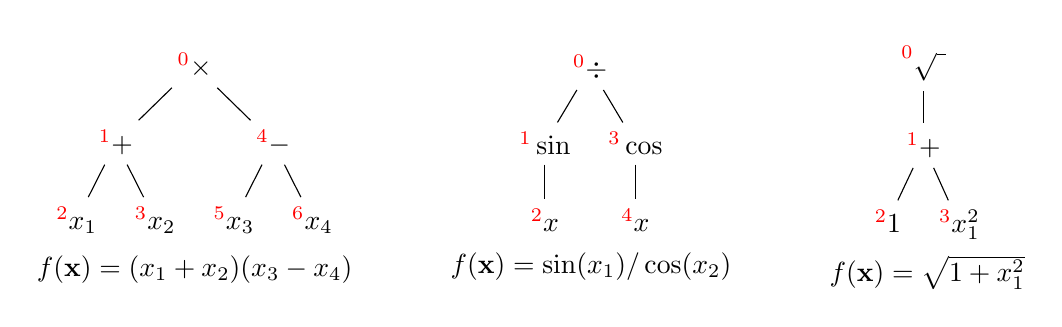
\begin{tikzpicture}
    \node[align=center] (n1) {
        \begin{forest}
            [$^{\color{red} 0}\times$ [$^{\color{red} 1}+$ [$^{\color{red}2}x_1$] [$^{\color{red}3}x_2$]] [$^{\color{red}4}-$ [$^{\color{red}5}x_3$] [$^{\color{red}6}x_4$]]]
        \end{forest}\\

        $f(\mathbf{x}) = (x_1 + x_2)(x_3 - x_4)$
    };

    \node[align=center, right=of n1] (n2) {
        \begin{forest}
            [ $^{\color{red} 0}\div$
                [ $^{\color{red} 1}\sin$ [$^{\color{red} 2}x$] ]
                [ $^{\color{red} 3}\cos$ [$^{\color{red} 4}x$] ]
            ]
        \end{forest}\\

        $f(\mathbf{x}) = \sin(x_1)/\cos(x_2)$
    };

    \node[align=center, right=of n2] (n3) {
        \begin{forest}
            [ $^{\color{red} 0}\sqrt{~}$
                [ $^{\color{red} 1}+$
                    [ $^{\color{red} 2}1$ ]
                    [ $^{\color{red} 3}x_1^2$ ]
                ]
            ]
        \end{forest}\\
        $f(\mathbf{x}) = \sqrt{1 + x_1^2}$
    };
\end{tikzpicture}

    \caption{Example tree representations with preorder traversal indices shown in red.}
    \label{fig:sr-tree-example}
\end{figure}

In GP-based SR, the tree representation encodes mathematical expressions, as illustrated in~\autoref{fig:sr-tree-example}. SR performs a search of the space of mathematical expressions by gradually assembling tree structures from a pre-configured set of functions and terminals.
%
Given a set of binary (e.g. $+, -, \times, \div, \mathrm{pow}, \mathrm{aq}, \dots$), unary (e.g. $\sin, \cos, \exp, \log, \sqrt{\cdot}, \dots$) and nullary (i.e. variables and parameters) operators, the search space is defined as all valid compositions of operators (subject to some size constraints), making it a discrete combinatorial search space whose dimension scales exponentially with the number of operators.

\begin{figure}
    \begin{subfigure}[b]{0.42\textwidth}
    \centering
    Parent tree $T_1$\\
    \begin{forest}
        [{$^{\color{red} 0}\times$}, name=n0
            [{$^{\color{red} 1}+$}, name=n1
                [{$^{\color{red}2}x_1$}, name=n2]
                [{$^{\color{red}3}x_2$}, name=n3]
            ]
            [{$^{\color{red}4}-$}, name=n4
                [{$^{\color{red}5}x_3$}, name=n5]
                [{$^{\color{red}6}x_4$}, name=n6]
            ]
        ]
        \begin{scope}[on background layer]
            \node[fill=orange!15, inner sep=0pt, rectangle, rounded corners, fit=(n4) (n5) (n6)] {};
        \end{scope}
    \end{forest}\\
    $f_1(\mathbf{x}) = (x_1 + x_2) \times (x_3 - x_4)$
\end{subfigure}
\begin{subfigure}[b]{0.29\textwidth}
    \centering
    Parent tree $T_2$\\
    \begin{forest}
        [{$^{\color{red} 0}\div$}, name=n0
            [{$^{\color{red} 1}\times$}, name=n1
                [{$^{\color{red}2}x_1$}, name=n2]
                [{$^{\color{red}3}x_2$}, name=n3]
            ]
            [{$^{\color{red}4}\centerdot^2$}, name=n4
                [{$^{\color{red}5}x_3$}, name=n5]
            ]
        ]
        \begin{scope}[on background layer]
            \node[fill=green!20, inner sep=0pt, rectangle, rounded corners, fit=(n4) (n5)] {};
        \end{scope}
    \end{forest}\\
    $f_2(\mathbf{x}) = {x_1 x_2}/{x_3^2}$
\end{subfigure}
\begin{subfigure}[b]{0.25\textwidth}
    \centering
    Child tree $C_1$\\
    \begin{forest}
        [{$^{\color{red} 0}\times$}, name=n0
            [{$^{\color{red} 1}+$}, name=n1
                [{$^{\color{red}2}x_1$}, name=n2]
                [{$^{\color{red}3}x_2$}, name=n3]
            ]
            [{$^{\color{red}4}\centerdot^2$}, name=n4
                [{$^{\color{red}5}x_3$}, name=n5]
            ]
        ]
        \begin{scope}[on background layer]
            \node[fill=green!20, inner sep=0pt, rectangle, rounded corners, fit=(n4) (n5)] {};
        \end{scope}
    \end{forest}\\
    $f_3(\mathbf{x}) = (x_1 + x_2){x_3^2}$
\end{subfigure}
    \caption{Crossover between two parent tree-encoded expressions. A new symbolic expression $f_3(\mathbf{x}) = (x_1 + x_2){x_3^2}$ is obtained by exchanging the parts $(x_3-x_4)$ and $x_3^2$ between the parents.}\label{fig:gp-crossover}
\end{figure}

The successful exploration of the search space depends on the existence of a sufficiently diverse set of individuals in the population, from which adaptive change can emerge as the product of recombination. At the same time, successful \textit{exploitation}, understood as the local improvement of solutions in the vicinity of optima points, requires a focusing of the search effort and depends on the selection mechanism's ability to concentrate the population on promising regions of the search space.
%
A balance between these two antagonistic aspects of the search is difficult to achieve since it requires a deep understanding of evolutionary dynamics and is, in general, problem-dependent~\cite{crepinsek2013}. A good trade-off depends on appropriate settings for parameters such as the population size, crossover and mutation probabilities or selection pressure. The latter plays a particularly important role, since it controls the survival and reproduction rates of fit individuals.

Selection in a finite population causes diversity loss due to duplication of fit individuals\cite{prugel-bennett2000}. In tournament selection, the most popular selection mechanism in SR, this effect was shown to be significant even at small tournament sizes\cite{xie2011}. A simulation of tournament selection in \autoref{fig:tournament-selection-pressure} shows that at least 40\% of individuals are lost in every generation.
%
Diversity has an impact on search convergence, as the outcome of recombination will depend on the amount of genetic material shared by the parents. The more similar the parents, the more likely a significant amount of duplicate material will be inherited by the child.

\begin{figure}
    \centering
    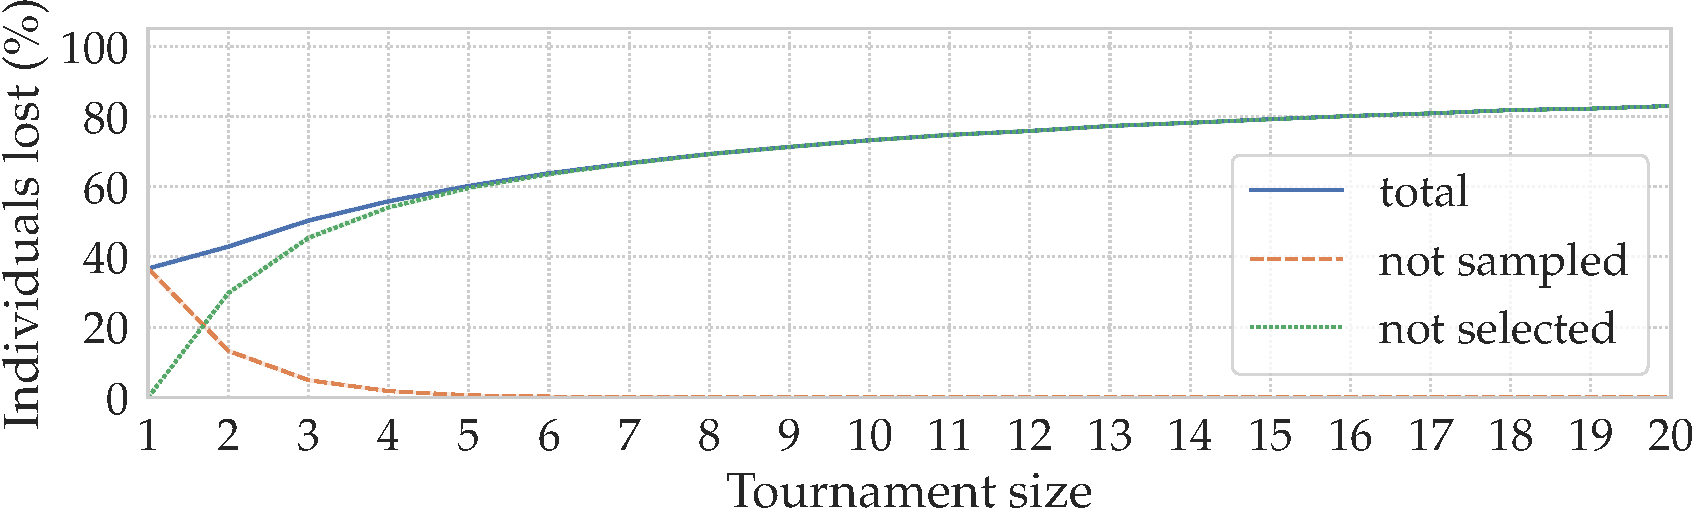
\includegraphics[width=0.8\textwidth]{./fig/tournament_selection_pressure.pdf}
    \caption{Percentage of not selected individuals as a function of tournament size}\label{fig:tournament-selection-pressure}
\end{figure}

From a practical perspective, given the unavoidable loss of diversity over the course of evolution, it is reasonable to assume that some solutions produced by recombination will not be unique, and their initial evaluations could be reused, with significant runtime benefits. Furthermore, detecting when duplicates \textit{may} occur or detecting the \textit{frequency} of duplicate individuals in the population may also lead to better strategies for diversity maintenance.
%

Previous attempts to improve runtime efficiency focused on alternative representations, for example storing the population as a graph\cite{handley1994,keijzer2004,defranca2025} or subtree caching\cite{wong2008}. The caching approach is of particular interest here as it does not require changes to the fundamental structure of the algorithm. However, implementing an efficient cache requires an accurate, low-overhead hashing function, with certain desirable properties such as hash involution. This paper introduces a hashing approach based on Zobrist keys that allows the caching of expression trees with minimal overhead, whose inner workings are described in the following section.


\section{Duplicate Detection in Symbolic Regression}\label{sec:duplicate-detection}

Duplicate detection in SR populations is challenging because of the need to compute distances between unordered labeled trees, a problem known to be NP-complete\cite{zhang1992}. However, if one relaxes the problem to approximate matching, then hash-based tree isomorphism offers similar results with a marginal error bounded by the collision rate\footnote{Perfect hashes are not considered due to their high computational cost.}. Hash functions based on modular arithmetic\cite{wong2008} or Merkle trees\cite{burlacu2019} have been previously used in SR to improve runtime and detect structural and semantic duplicates, but due to their logarithmic time complexity, their overhead remains significant.

Zobrist hashing, named after its inventor Albert Zobrist, is a hashing technique primarily used in computer game algorithms, particularly for board games such as Chess and Go.
%
At its core, Zobrist hashing involves assigning a unique random number to each possible piece on each possible square of the game board. For instance, in chess, each combination of piece type and board position is mapped to a distinct random number. The hash value of a particular board state is then computed by performing a bitwise XOR (exclusive OR) operation on the numbers corresponding to the pieces present on the board.

The Zobrist hash has excellent runtime properties as XOR operations are generally very well-optimized on modern CPUs due to their simplicity and suitability for parallel execution. But the main advantage of Zobrist hashing becomes apparent when considering the mathematical properties of the XOR function, namely associativity, commutativity and involution.
\begin{align*}
    a \oplus b &= b \oplus a & & \text{(associativity)}\\
    a \oplus (b \oplus c) &= (a \oplus b) \oplus c & & \text{(commutativity)}\\
    a \oplus b \oplus b &= a & & \text{(involution)}\\
\end{align*}
Given an abstract board game whose state can be reached through different move orders, the XOR function enables the incremental update of the game state by only considering changes to the board position after a move is made. In other words, previously visited states can be identified regardless of move order. This helps tree search algorithms such as \emph{Minimax} avoid already-visited nodes in the search tree, by maintaining a data structure called a \emph{transposition table} -- a database that stores results of previously performed searches -- greatly improving search efficiency.

The same approach is applicable to SR, considering the tree node type and its preorder index as the tabular coordinates for retrieving the associated Zobrist key, as illustrated in \autoref{fig:zobrist-tree-example}. When two parent trees are crossed-over, the child hash will not be recomputed but instead updated with the hashes of the swapped subtrees\footnote{The incremental update will be faster when the cumulated length of the swapped subtrees is smaller than the length of $T_1$.}. For example, the hash of the child individual from~\autoref{fig:gp-crossover} is obtained by:
\[
    \mathcal{H}(C_1) = \mathcal{H}(T_1) \oplus {\color{green!60!black}\underbrace{h_{-,4} \oplus h_{x_3,5} \oplus h_{x_4, 6}}_{\text{XOR ``out'' $(x_3 - x_4)$}}} \oplus {\color{blue} \underbrace{h_{\centerdot^2,4} \oplus  h_{x_3, 5}}_{\text{XOR ``in'' $x_3^2$}}}
\]

\begin{figure}
    \begin{subfigure}[b][3cm]{0.5\textwidth}
    Expression tree $T$

    \begin{forest}
        [{$^{\color{red} 0}\times$}, name=n0
            [{$^{\color{red} 1}+$}, name=n1
                [{$^{\color{red}2}x_1$}, name=n2]
                [{$^{\color{red}3}x_2$}, name=n3]
            ]
            [{$^{\color{red}4}-$}, name=n4
                [{$^{\color{red}5}x_3$}, name=n5]
                [{$^{\color{red}6}x_4$}, name=n6]
            ]
        ]
        \node[below=of n0, yshift=-1cm] {
            $f_1(\mathbf{x}) = (x_1 + x_2) \times (x_3 - x_4)$
        };
    \end{forest}
    \smallskip

    Prefix representation

    \begin{tabular}{ccccccc}
        $\times$ & $+$ & $x_1$ & $x_2$ & $-$ & $x_3$ & $x_4$\\
        0 & 1 & 2 & 3 & 4 & 5 & 6\\
    \end{tabular}

    \vspace{-2.33cm}
\end{subfigure}\begin{subfigure}[b][3cm]{0.5\textwidth}
    Zobrist table\smallskip

    \begin{tabular}{c|c}
        $+$ & \\
        $-$ & \\
        $\times$ & \\
        $\div$ & Filled with\\
        $\vdots$ & random values\\
        $\vdots$ & \\
        $\text{variable}$ & \\
        $\text{constant}$ & \\
        \hline
        & position $i = 0,\dots,N$\\
    \end{tabular}
\end{subfigure}\vspace{1.5em}
    \caption{$\mathcal{H}(T) = h_{\times,0} \oplus h_{+, 1} \oplus h_{x_1, 2} \oplus h_{x_2, 3} \oplus h_{-,4} \oplus h_{x_3, 5} \oplus h_{x_4, 6}$}
    \label{fig:zobrist-tree-example}
\end{figure}

% \subsubsection*{Zobrist-based Cache Implementation}

\subsubsection*{Implementation}

We are interested in implementing a cache that can store and retrieve the fitness values of visited solutions. The following components are necessary:

\paragraph{Zobrist table} The table is initialized with random values corresponding to each symbol $\times$ position combination, as illustrated in the right-hand side of figure~\autoref{fig:zobrist-tree-example}.
%
Its shape will be an $n\times l$ matrix where the number of symbols $n$ and the number of indices $l$ are given by:
\begin{align}
    n &= \underbrace{|\text{binary operators}| + |\text{unary operators|}}_\text{function nodes} + \underbrace{|\text{nullary operators}|}_\text{terminal nodes}\\
    l &= \text{the maximum tree length}
\end{align}
For example, if the primitive set contains $20$ symbols and the maximum tree length is $50$, then the Zobrist table will contain $1000$ values. To avoid hash collisions, we use 64-bit values generated with a high-quality pseudo-random number generator\footnote{We use the excellent general-purpose \texttt{xoshiro256**} generator from URL.}\cite{blackman2021}.

\paragraph{Zobrist hash function} The hash function iterates over tree nodes in preorder and aggregates the corresponding values from the Zobrist table using the XOR operation:
\begin{align}
    \mathcal{H}(T) = \bigoplus_{i=1}^{|T|} h\left( s_i, i \right)
\end{align}
where $T$ is a tree, $s_i$ is the symbol at position $i$ and $h(s_i, i)$ is a hash retrieval function:
\begin{align}
    h(s_i, i) = \begin{cases}
        \texttt{zobrist}(s_i, i) \oplus \texttt{id}(s_i) & \text{if $s_i$ is a variable} \\
        \texttt{zobrist}(s_i, i) & \text{otherwise}
    \end{cases}
\end{align}
%
In the case of variables, each Zobrist table value is XOR'd with a unique identifier associated with each variable. This definition of $h$ is necessary in order to treat variables as distinct symbols within this convention such that, for example, $\mathcal{H}({x_1}) \neq \mathcal{H}\left({x_2}\right)$.

Additionally, many SR implementations associate multiplicative coefficients with each tree node in order to enable a more granular fine-tuning of the model using local search. In this case, model coefficients can be included in the hash by XOR-ing their respective values into the corresponding node hash.

The cache is then implemented as a \texttt{hash\_map} object that maps Zobrist hash values to fitness. Integration with the workflow in~\autoref{fig:gp-workflow} is straightforward -- the logic needs to be slightly adapted to only re-evaluate a solution if it has not been cached before:

\begin{algorithmic}[1]
    \Procedure{Cached Fitness Evaluation}{$T$}
        \State $h \gets \mathcal{H}(T)$
        \If{$\texttt{cache}(h) = \emptyset$}
            \State $\texttt{cache}(h) \gets \textsc{EvaluateFitness}(T)$
        \EndIf
        \State \Return $\texttt{cache}(h)$
    \EndProcedure
\end{algorithmic}

As the most runtime critical part of the approach, the hash map implementation must be highly efficient and support concurrent read/write operations.
%
Our approach is integrated with the Operon library\cite{burlacu2020} which provides an efficient \CPP{} implementation of SR.

\section{Results}

We test the caching approach on a number of real-world datasets illustrated in~\autoref{tab:test-problems}.

\begin{table}
    \centering
    \begin{tblr}{
        colspec={lrrr},
        row{1} = {font=\bfseries}
    }
        Name & Features & Training size & Test size\\
        Chemical-I\cite{kordon2008} & 25 & 3136 & 1863\\
        Chemical-II\cite{kordon2008} & 57 & 711 & 355\\
        Flow stress\cite{kabliman2021} & 2 & 4200 & 3600\\
        FrictionDyn\cite{kronberger2018} & 17 & 1010 & 1016\\
        FrictionStat\cite{kronberger2018} & 16 & 1010 & 1016\\
        Nasa Battery 1\_10\cite{saha2007} & 6 & 504 & 132\\
        Nasa Battery 2\_20\cite{saha2007} & 5 & 1101 & 537\\
        Nikuradse-I\cite{nikuradse1950} & 2 & 230 & 132\\
        Nikuradse-II\cite{nikuradse1950} & 2 & 200 & 162\\
    \end{tblr}
    \caption{Test problems}\label{tab:test-problems}
\end{table}

\begin{figure}
    \centering

    \begin{subfigure}[b]{0.49\textwidth}
        \includegraphics[width=\textwidth]{./fig/global_diversity.pdf}
        \caption{Ratio of already-seen solutions}\label{fig:diversity}
    \end{subfigure}
    \begin{subfigure}[b]{0.49\textwidth}
        \includegraphics[width=\textwidth]{./fig/evaluation_count.pdf}
        \caption{Solution evaluations}\label{fig:evaluation-count}
    \end{subfigure}
    % \caption{Evolution of structural diversity}
    % \label{fig:diversity}
\end{figure}

\begin{table}
    \SetTblrInner{colsep=5pt}
\begin{tblr}{colspec={X[l]ccccc},
        row{1,2} = {font=\bfseries},
        cell{1}{2} = {c=5}{c},
        cell{1}{1} = {c=1}{l},
        row{even}={bg=abstractcolor},
        row{1}={bg=abstractcolor},
        cell{4}{3,4,5,6} = {bg=green!20!abstractcolor}, % mark better
        cell{6}{3} = {bg=green!20!abstractcolor},
        cell{8}{4,5,6} = {bg=green!20!abstractcolor},
        cell{8}{2,3} = {bg=red!15!abstractcolor},
        cell{10,12}{2} = {bg=red!15!abstractcolor},
        cell{10}{3,4,5,6} = {bg=green!20!abstractcolor},
        cell{14}{3,4,5,6} = {bg=green!20!abstractcolor},
        cell{16}{5} = {bg=red!15!abstractcolor},
        cell{16}{2} = {bg=green!20!abstractcolor},
        cell{18}{5} = {bg=green!20!abstractcolor},
        cell{20}{3} = {bg=green!20!abstractcolor}
        % cell{2}{3,5,7,9,11} = {c=2}{c},
        % cell{3,5}{1} = {font=\bfseries}
        % cell{8}{1} = {r=2}{c}
    }
% WORSE
% Flow-stress 0 0.9434521794319153 0.9509314298629761 0.0003199486402201191
% Flow-stress 1 0.9477692246437073 0.950948566198349 0.0013689616910057645
% FrictionDyn-OneHot 0 0.6348792314529419 0.7228361368179321 2.5843478684547606e-07
% FrictionStat-OneHot 0 0.26015421748161316 0.2941109836101532 2.4246659410859725e-07
% Nasa Battery 2h 20min 50 0.9708788096904755 0.9722806513309479 0.04138746154555723

% BETTER
% Chemical-I 1 0.9124540388584137 0.9097577631473541 0.007994153730759613
% Chemical-I 10 0.9219879508018494 0.9196093678474426 2.5483324299701395e-05
% Chemical-I 50 0.9225679934024811 0.9191929697990417 2.1056811737961928e-08
% Chemical-I 100 0.9216791391372681 0.9198945462703705 0.0005485318623525329
% Chemical-II 1 0.8269909024238586 0.8081256747245789 0.0003193350354699925
% Flow-stress 10 0.9987938106060028 0.9985659420490265 0.0048498858303766094
% Flow-stress 50 0.9990395605564117 0.9989723265171051 0.008545048537085678
% Flow-stress 100 0.9990545511245728 0.9989436864852905 7.598858495256795e-07
% FrictionDyn-OneHot 1 0.8686016499996185 0.8560784161090851 1.3695168136253396e-05
% FrictionDyn-OneHot 10 0.8689292967319489 0.8647867441177368 0.0016992309412517767
% FrictionDyn-OneHot 50 0.8722218573093414 0.8631846606731415 3.841875961442836e-11
% FrictionDyn-OneHot 100 0.8712080717086792 0.8677948713302612 2.383564486694608e-05
% Nasa Battery 1h 10min 1 0.9934685528278351 0.9922453165054321 8.850301987032161e-07
% Nasa Battery 1h 10min 10 0.9938161075115204 0.992877870798111 0.0012137034566344373
% Nasa Battery 1h 10min 50 0.9938184916973114 0.9931999742984772 0.0013750472222200686
% Nasa Battery 1h 10min 100 0.9939332008361816 0.9927870035171509 7.5076634927637944e-06
% Nasa Battery 2h 20min 0 0.9783627390861511 0.978304922580719 0.020226707636176792
% Nikuradse-I 50 0.992519348859787 0.9893010258674622 6.569295257622376e-06
% Nikuradse-II 1 0.9824371337890625 0.9823247492313385 0.0026725298155811958
        Problem            & Local Search Iterations & & & & \\
                           & 0                               & 1                               & 10                              & 50                              & 100 \\
        Chemical-I & $\num{0.8173} \pm \num{0.0826}$ & $\num{0.9098} \pm \num{0.0091}$ & $\num{0.9196} \pm \num{0.0046}$ & $\num{0.9192} \pm \num{0.0046}$ & $\num{0.9199} \pm \num{0.0064}$\\
 & $\num{0.8352} \pm \num{0.0660}$ & $\num{0.9125} \pm \num{0.0062}$ & $\num{0.9220} \pm \num{0.0031}$ & $\num{0.9226} \pm \num{0.0032}$ & $\num{0.9217} \pm \num{0.0035}$\\
        Chemical-II & $\num{0.5527} \pm \num{0.1190}$ & $\num{0.8081} \pm \num{0.0822}$ & $\num{0.8020} \pm \num{0.1207}$ & $\num{0.7881} \pm \num{0.1639}$ & $\num{0.7943} \pm \num{0.1259}$\\
        & $\num{0.5690} \pm \num{0.1279}$ & $\num{0.8270} \pm \num{0.0399}$ & $\num{0.8050} \pm \num{0.0754}$ & $\num{0.8013} \pm \num{0.1290}$ & $\num{0.8066} \pm \num{0.1313}$\\
        Flow-stress & $\num{0.9509} \pm \num{0.0452}$ & $\num{0.9509} \pm \num{0.0426}$ & $\num{0.9986} \pm \num{0.1445}$ & $\num{0.9990} \pm \num{0.0712}$ & $\num{0.9989} \pm \num{0.1174}$\\
        & $\num{0.9435} \pm \num{0.1032}$ & $\num{0.9478} \pm \num{0.0482}$ & $\num{0.9988} \pm \num{0.1010}$ & $\num{0.9990} \pm \num{0.0870}$ & $\num{0.9991} \pm \num{0.0230}$\\
        FrictionDyn & $\num{0.7228} \pm \num{0.0773}$ & $\num{0.8561} \pm \num{0.0254}$ & $\num{0.8648} \pm \num{0.0069}$ & $\num{0.8632} \pm \num{0.0143}$ & $\num{0.8678} \pm \num{0.0069}$\\
        & $\num{0.6349} \pm \num{0.1201}$ & $\num{0.8686} \pm \num{0.0082}$ & $\num{0.8689} \pm \num{0.0061}$ & $\num{0.8722} \pm \num{0.0043}$ & $\num{0.8712} \pm \num{0.0049}$\\
        FrictionStat & $\num{0.2941} \pm \num{0.1862}$ & $\num{0.8427} \pm \num{0.1491}$ & $\num{0.8533} \pm \num{0.0457}$ & $\num{0.8625} \pm \num{0.0164}$ & $\num{0.8584} \pm \num{0.0274}$\\
        & $\num{0.2602} \pm \num{0.2223}$ & $\num{0.8432} \pm \num{0.1513}$ & $\num{0.8524} \pm \num{0.0682}$ & $\num{0.8629} \pm \num{0.0134}$ & $\num{0.8605} \pm \num{0.0215}$\\
        Nasa Bat 1\_10 & $\num{0.9832} \pm \num{0.0086}$ & $\num{0.9922} \pm \num{0.0036}$ & $\num{0.9929} \pm \num{0.0033}$ & $\num{0.9932} \pm \num{0.0039}$ & $\num{0.9928} \pm \num{0.0030}$\\
        & $\num{0.9856} \pm \num{0.0122}$ & $\num{0.9935} \pm \num{0.0015}$ & $\num{0.9938} \pm \num{0.0023}$ & $\num{0.9938} \pm \num{0.0018}$ & $\num{0.9939} \pm \num{0.0018}$\\
        Nasa Bat 2\_20 & $\num{0.9783} \pm \num{0.0678}$ & $\num{0.9724} \pm \num{0.0161}$ & $\num{0.9712} \pm \num{0.0047}$ & $\num{0.9723} \pm \num{0.0042}$ & $\num{0.9716} \pm \num{0.0049}$\\
        & $\num{0.9784} \pm \num{0.0528}$ & $\num{0.9727} \pm \num{0.0040}$ & $\num{0.9710} \pm \num{0.0051}$ & $\num{0.9709} \pm \num{0.0046}$ & $\num{0.9732} \pm \num{0.0047}$\\
        Nikuradse-I & $\num{0.8908} \pm \num{0.1314}$ & $\num{0.9207} \pm \num{0.1888}$ & $\num{0.9863} \pm \num{0.2081}$ & $\num{0.9893} \pm \num{0.1399}$ & $\num{0.9923} \pm \num{0.1253}$\\
        & $\num{0.8817} \pm \num{0.1342}$ & $\num{0.9440} \pm \num{0.1862}$ & $\num{0.9867} \pm \num{0.1326}$ & $\num{0.9925} \pm \num{0.0304}$ & $\num{0.9930} \pm \num{0.0582}$\\
        Nikuradse-II & $\num{0.9728} \pm \num{0.1236}$ & $\num{0.9823} \pm \num{0.0339}$ & $\num{0.9824} \pm \num{0.0199}$ & $\num{0.9824} \pm \num{0.1357}$ & $\num{0.9824} \pm \num{0.0438}$\\
        & $\num{0.9722} \pm \num{0.1564}$ & $\num{0.9824} \pm \num{0.0076}$ & $\num{0.9825} \pm \num{0.0002}$ & $\num{0.9824} \pm \num{0.1171}$ & $\num{0.9824} \pm \num{0.1357}$\\
    \end{tblr}
    \caption{Test performance expressed as median test $R^2 \pm \sigma$}
\end{table}

% \begin{table}
%     \input{./fig/best_length_mdl.tex}
%     \caption{Average length of the best solution $\pm \sigma$}
% \end{table}

% \newpage % remove me
\bibliographystyle{RS}
\bibliography{references}

\end{document}